\documentclass{beamer}
\mode<presentation>
\usepackage{amsmath}
\usepackage{amssymb}
%\usepackage{advdate}
\usepackage{graphicx}
\graphicspath{{../figs/}}
\usepackage{adjustbox}
\usepackage{subcaption}
\usepackage{enumitem}
\usepackage{multicol}
\usepackage{mathtools}
\usepackage{listings}
\usepackage{url}
\def\UrlBreaks{\do\/\do-}
\usetheme{Boadilla}
\usecolortheme{lily}
\setbeamertemplate{footline}
{
  \leavevmode%
  \hbox{%
  \begin{beamercolorbox}[wd=\paperwidth,ht=2.25ex,dp=1ex,right]{author in head/foot}%
    \insertframenumber{} / \inserttotalframenumber\hspace*{2ex} 
  \end{beamercolorbox}}%
  \vskip0pt%
}
\setbeamertemplate{navigation symbols}{}
\let\solution\relax
\usepackage{gvv}
\lstset{
%language=C,
frame=single, 
breaklines=true,
columns=fullflexible
}

\numberwithin{equation}{section}



\begin{document}

\title{4.13.25}
\author{EE25BTECH11020 - Darsh Pankaj Gajare}
% \maketitle
% \newpage
% \bigskip
%\begin{document}
{\let\newpage\relax\maketitle}
%\renewcommand{\thefigure}{\theenumi}
%\renewcommand{\thetable}{\theenumi}
Question:\\
Two sides of a rhombus are along the lines, $x - y + 1 = 0$ and $7x - y - 5 = 0$. If its diagonals intersect at $\brak{-1, -2}$, then which one of the following is a vertex of this rhombus?
\begin{enumerate}[label=(\Alph*)]
		\begin{multicols}{4}
		\item $\brak{\frac{1}{3},-\frac{8}{3}}$
		\item $\brak{-\frac{10}{3},-\frac{7}{3}}$
		\item $\brak{-3,-9}$
		\item $\brak{-3,-8}$
		\end{multicols}
\end{enumerate}
\solution
\begin{table}[H]
	\centering
	\caption{}
	\begin{tabular}{|c|c|}
\hline
\textbf{Name} & \textbf{Value} \\ \hline
$\vec{A}$ & $\myvec{2 & 1 \\0 & 3}$ \\ \hline
\end{tabular}

	\label{}
\end{table}
\begin{align}
A\vec{V_A} &= b, \quad 
A=\myvec{1 & -1\\ 7 & -1},\ 
b=\myvec{-1\\ 5} \\ 
\augvec{2}{1}{1 & -1 & -1\\ 7 & -1 & 5} 
&\xrightarrow{R_2-7R_1} 
\augvec{2}{1}{1 & -1 & -1\\ 0 & 6 & 12} \\ 
\vec{V_A} &= \myvec{1\\2} 
\end{align}

\begin{align}
\vec{V_C} &= 2\vec{O}-\vec{V_A}
=2\myvec{-1\\-2}-\myvec{1\\2}
=\myvec{-3\\-6}
\end{align}

\begin{align}
k &= -\vec{n_1}^T\vec{V_C}=-3, \quad
m=-\vec{n_2}^T\vec{V_C}=15
\end{align}

\begin{align}
\augvec{2}{1}{1 & -1 & 3\\ 7 & -1 & 5}
&\xrightarrow{R_2-7R_1}
\augvec{2}{1}{1 & -1 & 3\\ 0 & 6 & -16} \\ 
\vec{V} &= \myvec{\frac{1}{3}\\ -\frac{8}{3}} \\ 
\end{align}\begin{figure}[H]
	\centering
	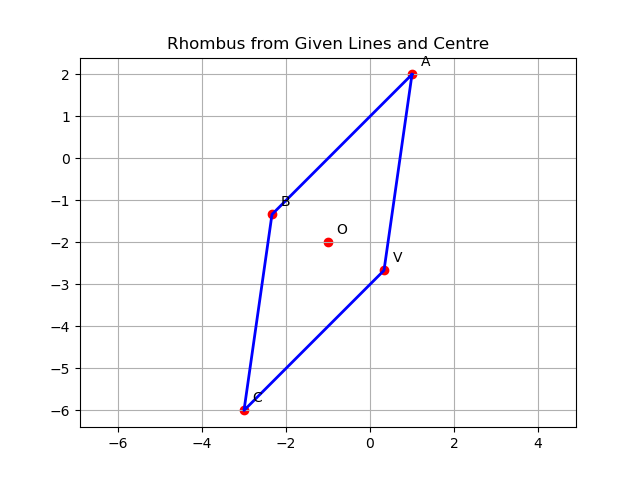
\includegraphics[scale=0.25]{img1}
	\caption*{Plot using C libraries}
	\label{img1}
\end{figure}
\begin{figure}[H]
	\centering
	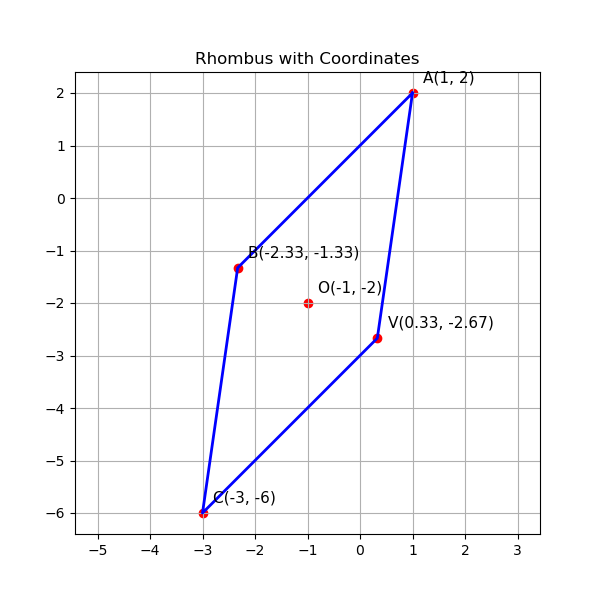
\includegraphics[scale=0.25]{img2}
	\caption*{Plot using Python}
	\label{img2}
\end{figure}
\end{document}

